% Template for PLoS
% Version 3.1 February 2015
%
% To compile to pdf, run:
% latex plos.template
% bibtex plos.template
% latex plos.template
% latex plos.template
% dvipdf plos.template
%
% % % % % % % % % % % % % % % % % % % % % %
%
% -- IMPORTANT NOTE
%
% This template contains comments intended 
% to minimize problems and delays during our production 
% process. Please follow the template instructions
% whenever possible.
%
% % % % % % % % % % % % % % % % % % % % % % % 
%
% Once your paper is accepted for publication, 
% PLEASE REMOVE ALL TRACKED CHANGES in this file and leave only
% the final text of your manuscript.
%
% There are no restrictions on package use within the LaTeX files except that 
% no packages listed in the template may be deleted.
%
% Please do not include colors or graphics in the text.
%
% Please do not create a heading level below \subsection. For 3rd level headings, use \paragraph{}.
%
% % % % % % % % % % % % % % % % % % % % % % %
%
% -- FIGURES AND TABLES
%
% Please include tables/figure captions directly after the paragraph where they are first cited in the text.
%
% DO NOT INCLUDE GRAPHICS IN YOUR MANUSCRIPT
% - Figures should be uploaded separately from your manuscript file. 
% - Figures generated using LaTeX should be extracted and removed from the PDF before submission. 
% - Figures containing multiple panels/subfigures must be combined into one image file before submission.
% For figure citations, please use "Fig." instead of "Figure".
% See http://www.plosone.org/static/figureGuidelines for PLOS figure guidelines.
%
% Tables should be cell-based and may not contain:
% - tabs/spacing/line breaks within cells to alter layout or alignment
% - vertically-merged cells (no tabular environments within tabular environments, do not use \multirow)
% - colors, shading, or graphic objects
% See http://www.plosone.org/static/figureGuidelines#tables for table guidelines.
%
% For tables that exceed the width of the text column, use the adjustwidth environment as illustrated in the example table in text below.
%
% % % % % % % % % % % % % % % % % % % % % % % %
%
% -- EQUATIONS, MATH SYMBOLS, SUBSCRIPTS, AND SUPERSCRIPTS
%
% IMPORTANT
% Below are a few tips to help format your equations and other special characters according to our specifications. For more tips to help reduce the possibility of formatting errors during conversion, please see our LaTeX guidelines at http://www.plosone.org/static/latexGuidelines
%
% Please be sure to include all portions of an equation in the math environment.
%
% Do not include text that is not math in the math environment. For example, CO2 will be CO\textsubscript{2}.
%
% Please add line breaks to long display equations when possible in order to fit size of the column. 
%
% For inline equations, please do not include punctuation (commas, etc) within the math environment unless this is part of the equation.
%
% % % % % % % % % % % % % % % % % % % % % % % % 
%
% Please contact latex@plos.org with any questions.
%
% % % % % % % % % % % % % % % % % % % % % % % %

\documentclass[10pt,letterpaper]{article}
\usepackage[top=0.85in,left=2.75in,footskip=0.75in]{geometry}

% Use adjustwidth environment to exceed column width (see example table in text)
\usepackage{changepage}

% Use Unicode characters when possible
\usepackage[utf8]{inputenc}

% textcomp package and marvosym package for additional characters
\usepackage{textcomp,marvosym}

% fixltx2e package for \textsubscript
\usepackage{fixltx2e}

% amsmath and amssymb packages, useful for mathematical formulas and symbols
\usepackage{amsmath,amssymb}

% cite package, to clean up citations in the main text. Do not remove.
\usepackage{cite}

% Use nameref to cite supporting information files (see Supporting Information section for more info)
\usepackage{nameref,hyperref}

% line numbers
\usepackage[right]{lineno}

% ligatures disabled
\usepackage{microtype}
\DisableLigatures[f]{encoding = *, family = * }

% rotating package for sideways tables
\usepackage{rotating}

\usepackage{verbatim}   % useful for program listings

% Remove comment for double spacing
%\usepackage{setspace} 
%\doublespacing

% Text layout
\raggedright
\setlength{\parindent}{0.5cm}
\textwidth 5.25in 
\textheight 8.75in

% Bold the 'Figure #' in the caption and separate it from the title/caption with a period
% Captions will be left justified
\usepackage[aboveskip=1pt,labelfont=bf,labelsep=period,justification=raggedright,singlelinecheck=off]{caption}

% Use the PLoS provided BiBTeX style
\bibliographystyle{plos2015}

% Remove brackets from numbering in List of References
\makeatletter
\renewcommand{\@biblabel}[1]{\quad#1.}
\makeatother

% Leave date blank
\date{}

% Header and Footer with logo
\usepackage{lastpage,fancyhdr,graphicx}
\usepackage{epstopdf}
\pagestyle{myheadings}
\pagestyle{fancy}
\fancyhf{}
\lhead{\includegraphics[width=2.0in]{PLOS-submission.eps}}
\rfoot{\thepage/\pageref{LastPage}}
\renewcommand{\footrule}{\hrule height 2pt \vspace{2mm}}
\fancyheadoffset[L]{2.25in}
\fancyfootoffset[L]{2.25in}
\lfoot{\sf PLOS}

%% Include all macros below

\newcommand{\lorem}{{\bf LOREM}}
\newcommand{\ipsum}{{\bf IPSUM}}

%% END MACROS SECTION


\begin{document}
\vspace*{0.35in}

% Title must be 250 characters or less.
% Please capitalize all terms in the title except conjunctions, prepositions, and articles.
\begin{flushleft}
{\Large
\textbf\newline{Filament Recycling and Sustained Contractile Flows in an Actomyosin Cortex}
}
\newline
% Insert author names, affiliations and corresponding author email (do not include titles, positions, or degrees).
\\
William McFadden\textsuperscript{1},
Jonathan Michaux\textsuperscript{2},
Patrick McCall\textsuperscript{3},
Edwin Munro\textsuperscript{2,*}
\\
\bigskip
\bf{1} Biophysical Sciences Program, University of Chicago, Chicago, IL, USA
\\
\bf{2} Department of Molecular Genetics and Cell Biology, University of Chicago, Chicago, IL, USA
\\
\bf{3} Department of Physics, University of Chicago, Chicago, IL, USA
\\
\bigskip

% Insert additional author notes using the symbols described below. Insert symbol callouts after author names as necessary.
% 
% Remove or comment out the author notes below if they aren't used.
%
% Primary Equal Contribution Note
%\Yinyang These authors contributed equally to this work.

% Additional Equal Contribution Note
% Also use this double-dagger symbol for special authorship notes, such as senior authorship.
%\ddag These authors also contributed equally to this work.

% Current address notes
%\textcurrency a Insert current address of first author with an address update
% \textcurrency b Insert current address of second author with an address update
% \textcurrency c Insert current address of third author with an address update

% Deceased author note
%\dag Deceased

% Group/Consortium Author Note
%\textpilcrow Membership list can be found in the Acknowledgments section.

% Use the asterisk to denote corresponding authorship and provide email address in note below.
* emunro@uchicago.edu

\end{flushleft}
% Please keep the abstract below 300 words
\section*{Abstract}
Fill in abstract later.


% Please keep the Author Summary between 150 and 200 words
% Use first person. PLOS ONE authors please skip this step. 
% Author Summary not valid for PLOS ONE submissions.   
\section*{Author Summary}
In this paper, we develop and analyze a minimal model for 2D active networks based on the cortical cytoskeleton of eukaryotic embryos.  Our model introduces a drag-like slip between cross-linked filaments as means to dissipate stored stress, generating a macroscopic effective viscosity.  We further introduce an active friction to active stress from microscopic properties.  We generate computational simulations based on the model, and demonstrate that active stress is sufficient to drive network contraction only temporarily.  By introducing filament recycling, we are able to set up steady state flow profiles such as those found in the cortex of developing embryos and migrating cells.  The model is used to calculate phenomenological constants measured in prior experiments.  Our analysis sheds insight on potential microscopic control parameters governing broad qualitative differences in 2D active networks.  We make our model freely accessible and our methodology transparent to enable other researchers to clearly understand our modeling framework and to build upon our findings.

\linenumbers

\section*{Introduction}

\paragraph{Cortical flow is a fundamental process in cells, important for cell polarization, cell motility, and embryonic development \cite{cellmech_flows3,cellmech_flows2}.}  This fundamental ability to move and change shape depends on the actomyosin cortex, a thin layer of cross-linked actin filaments and myosin motors that lies just beneath the plasma membrane.  In this cortical layer, the interplay of myosin motor activity pulling against cross-linked actin filaments is able to drive these long range flows\cite{Munro2004413}, though this process is still not well understood.  Importantly, the actomyosin cortex is highly dynamic; filaments are disassembled and reassembled continuously, with a typical monomer lifetime of just tens of seconds. Dynamic filament recycling is essential to allow remodelling of cellular structure during development and physiology, but how this works remains poorly understood as well. Here, we focus on exploring how dynamic cross-links and actin filament recycling can tune rates of network deformation to allow cells to generate steady-state actomyosin flows, which are a crucial element of cell polarization and cell migration.

\paragraph{Cortical flows arise from active motors generating stresses in a viscously relaxing network.}  Our current understanding of the physics of cortical flows arises from the physics of active fluids\cite{cellmech_flows}.  In this model, the pattern of flow arises in response to gradients in internal active stress arising from local imbalances in active motor concentration\cite{PhysRevLett.106.028103}.  These theories have had much success in explaining macroscopic patterns such as the formation of contractile rings\cite{PhysRevLett.103.058102}.  Both active stress and passive relaxation will be highly dependent on a microscopic parameters such as network density and turnover rates, and there has already been a great deal of work done one deriving the microscopic scale understanding of contractile actin networks.  However, there is still a gap between how these microscopic parameters relate to local properties and what influence this will have on large-scale macroscopic flows.   Our aim is to build a minimal microscopic model of an active, cross-linked filament network with turnover that will allow us to draw direct comparisons to macroscopic levels of stress buildup, stress relaxation, and cortical flow velocity.


\paragraph{At long timescales, cross-linked filament networks relax their internal stresses.} Fluid-like stress relaxation have been observed in a number of cellular processes\cite{cellmech_flows,cellmech_flows2,cellmech_flows3,rheo_fluid,rheo_fluid2,cell_rheo_exp}.  These modes of stress relaxation are predominantly believed to arise from both the transient binding of cross-links and from the rapid turnover of filaments.  In {\em in vitro} studies, long timescale creep behaviors are thought to arise predominantly from the transient nature of filament binding for most biologically relevant cross-linkers\cite{rheo_crosslinksmatter,rheo_crosslinkslip1,rheo_crosslinkslip2,rheo_crosslinkslip3,rheo_nonaffine}.  However, the rapid rates of stress relaxation needed to produce large scale cell shape changes have made it clear that rapid actin turnover must play a significant role as well.  Indeed, energy consuming biochemical processes drive the rapid disassembly and reassembly of actin filaments, through a process we call filament recycling.   Although several theoretical methods have addressed cross-link binding and unbinding analytically \cite{theo_crosslinkslip1,theo_crosslinkslip2} and others have explicitly modeled reversible cross-linking in combination with complex mechanics of filament bundles\cite{model_taeyoon,rheo_crosslinkslip2,theo_crosslinkslip3}, less attention has been paid to actin turnover as mechanism of stress relaxation. However, recent efforts have begun to the fluid like properties of networks under applied stresses\cite{Kim2014526}, and some experimental work is beginning to elucidate their mechanical properties [Cite McCall].

\paragraph{Current understanding of stress generation in disordered active networks }

The coordinated action of actin and myosin alone has been show to be sufficient to drive contraction in synthetic systems\cite{rheo_2D1}.  Filament extensional asymmetry and dispersion in motor activity are sufficient conditions for the contraction in one \cite{1367-2630-14-3-033037} and two \cite{PhysRevX.4.041002} dimensional networks.  Further work has explored a multitude of microscopic parameters that can tune contractile patterns \cite{10.1371/journal.pone.0039869,Alvarado:2013aa,C0SM00494D} or mechanical properties of networks \cite{0295-5075-85-1-18007,rheo_active}.  However all of these examples generate momentary contraction which eventually stalls.  More recent efforts have begun to elucidate how network turnover can generate sustained flows\cite{10.1371/journal.pone.0000696}, and several modeling efforts have begun to view how long term stalling can be avoided in the presence of filament turnover \cite{2015arXiv150706182H,Mak:2016aa}. These systems of contractile material with turnover can generate highly dynamic behaviors\cite{PhysRevLett.113.148102}, but much work remains to understand the general principles underlying these results.

\paragraph{Our model allows calculation of results at long-timescales while incorporating a coarse-grained micro-scale model.}  
To incorporate as much micro-scale detail as possible while still maintaining the generality of the active fluid theory, we introduce several coarse-grained approximations into our representation of filament networks.  First, we simplify the complex asymmetric compliance of semi-flexible polymers with a simple asymmetric spring compliance.  Second, we simplify cross-linking via filament drag-like coupling in which filaments are able to slide past each other as molecular bonds form and rupture, akin to coarse-grained models of molecular friction\cite{theo_friction,theo_frictionSam,theo_molefric}.  Third, our networks are imbued with dispersion of activity by making a subset of filament overlaps into "active" cross-links\cite{theo_frictionShila}.  Finally, we generate filament turnover by regularly reseting a subset of filaments to a new unstrained position.  Importantly, these simplification allows us to extend our single polymer models to dynamical systems of larger network models for direct comparison between theory and modeling results.  This level of coarse graining will therefore make it easier to understand classes of behavior for varying compositions of cross-linked filament networks.  In addition, it allows us to compute a new class of numerical simulations efficiently, which gives us concrete predictions for behaviors in widely different networks with measurable dependencies on molecular details.

  

\paragraph{We have used our model to investigate how rates of flow will depend on microscopic properties of networks.}
Another quick summary which will be easy after the paper is written. 


% You may title this section "Methods" or "Models". 
% "Models" is not a valid title for PLoS ONE authors. However, PLoS ONE
% authors may use "Analysis" 
\section*{Models}

\begin{figure}[h!]
\centering
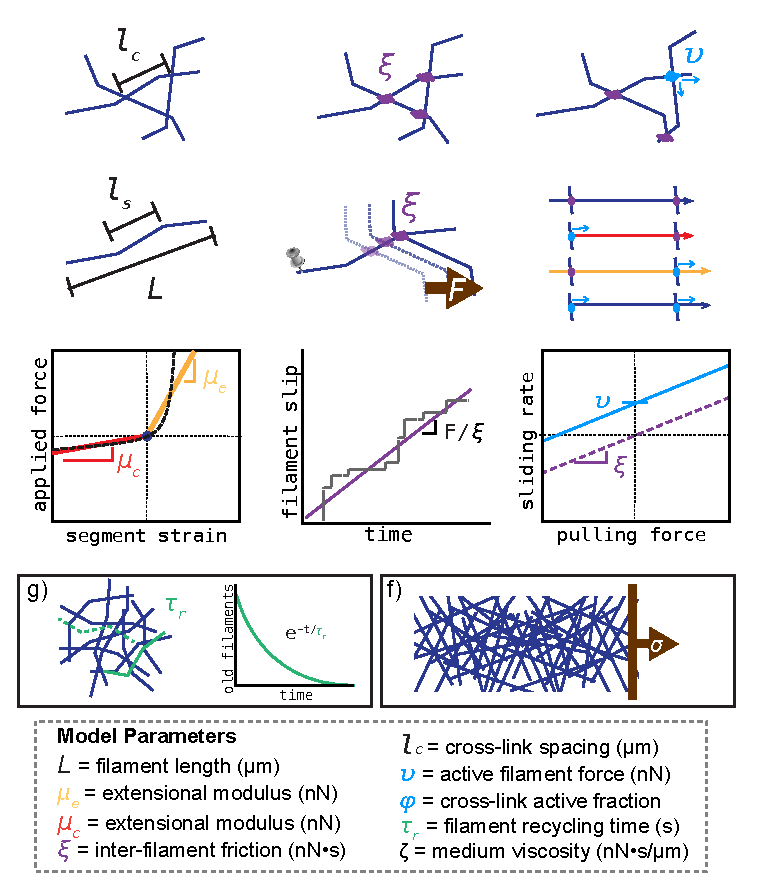
\includegraphics[width=\hsize]{figures/fig2/fig2}
\caption{\label{fig:sim} Schematic of modeling framework. a) Asymmetric filament compliance.  Filaments have smaller spring constant for compression than for extension. b) Cross-link slip.  Cross-links are coupled by an effective drag, such that their relative motion is proportional to any applied force. c) Motor activity. Filament activity manifests as a basal sliding rate even in the absence of an external force. d) Fractional activity.  Only a subset of filament cross-links are active, resulting in differential force exertion along the filament.  e)  Filament recycling.  Filaments are turned over at a constant rate, leading to a refreshing in the strain state of all filaments after a characteristic timescale.}
\end{figure}

We choose to focus our attention on 2D networks both for their tractability as well as their relevance in the quasi-2D cytoskeletal cortex of many eukaryotic cells\cite{cellmech_flows}.  In addition, recent developments in 2D {\em in vitro} systems\cite{rheo_2D1,rheo_2D2}, make 2D disordered models all the more interesting as a renewed focus of study.  In the rest of this section, we underline the key points necessary for understanding our modeling framework and the key assumptions we have made in generating our equations of motion for the system.


\subsection*{Asymmetric Filament Compliance}
We model individual filaments as chains of springs with relaxed length $l_s$.  Filaments can therefore be represented as a sequence of nodes with positions $\mathbf{x_i}$ and nearest neighbor force interactions, $\mathbf{F_i}$, of the form

\begin{equation}
|F_i| = \mu\cdot\frac{|\mathbf{x_{i+1}}-\mathbf{x_i}|-l_s}{l_s} +\mu\cdot\frac{|\mathbf{x_{i-1}}-\mathbf{x_i}|-l_s}{l_s}
\end{equation}





where, $\mu$ represents an extensional modulus of a filament.   Here, we take the modulus, $\mu$, to have a different value depending on whether $|\mathbf{x_{i-1}}-\mathbf{x_i}|-l_s$ is greater or less than 0.  This moduli is a composite quantity related to both filament and cross-linker compliance in a manner similar to a proposed effective medium theory\cite{theo_crosslinknonlinear}.  In the limit of highly rigid cross-links and flexible filaments, our model reduces to the pure semi-flexible filament models of \cite{theo_hlm,theo_hlm2}.  In the opposite regime of nearly rigid filaments and highly flexible cross links, our method is still largely similar to the model of \cite{theo_crosslinknonlinear} in small strain regimes before any nonlinear cross link stiffening.  However, in departure from those models, the magnitude of the force on interior cross-links in our model is still the same as those on the exterior.  This is a simplification of the varying levels of strain that would actually be present in these cross-linkers as addressed in \cite{theo_crosslinknonlinear}, but we choose to ignore the slight variation in favor of an approximated, global mean approach.  



\subsection*{Drag-like Coupling Between Overlapping Filaments}
\label{exp_drag}
Cross-link binding and unbinding is an important element of the overall stress relaxation of a network.  In contrast to previous models, we allow relaxation of the network's stored stress by letting the attachment points slip.  We do this by replacing an elastic interaction between pairs of points along filament segments with a drag-like coupling between segments.
\begin{equation}
\mathbf{F_{drag}} = \xi \cdot \int ds \: (\mathbf{v_i(s)}-\mathbf{v_j(s)}) \: p_{ij}(s)
\end{equation}

Where $p_{ij}(s)$ represents the locational distribution of cross-link points (equal to 1 at locations of cross-links and 0 elsewhere) and $\mathbf{v_i(s)}$ and $\mathbf{v_j(s)}$ represent the the velocities of the $i$th and $j$th filament segment.  This model assumes a linear relation between applied force and the velocity difference between attached segments.  This drag-like coupling has been shown to be an adequate approximation in the case of ionic cross-linking of actin\cite{mol_fric,theo_hydroish2}, and can be found in the theoretical basis of force-velocity curves for myosin bound filaments\cite{theo_frictionShila}. Although non-linearities can arise through force dependent detachment kinetics and/or non-linear force extension of cross-links, we assume that inhomogeneities from non-linear effects are of second or higher order. With this assumption, the motion for the entire network is governed by a dynamical equation of the form

\begin{equation}
\label{eqn:syst}
\int ds \: (\mathbf{\zeta v_i(s)} + \xi \sum _j(\mathbf{v_i(s)}-\mathbf{v_j(s)}) \: p_{ij}(s))= \mathbf{F_i}
\end{equation}

Here, the first term in the integral is the filament's intrinsic drag through its embedding fluid, $\zeta$, while the second comes from the drag-like coupling between filaments, $\xi$.  

\subsection*{Active Coupling for Motor Driven Filament Interactions}

To add motor activity we select a subset of cross-linked points and impart an additional force of magnitude $\upsilon$ directed in the orientations of the individual filaments, $\mathbf{u_i}$.  This leads to a modification of the equation of motion to

\begin{equation}
\label{eqn:syst}
\int ds \: (\mathbf{\zeta v_i(s)} + \xi \sum _j(\mathbf{v_i(s)}-\mathbf{v_j(s)}) \: p_{ij}(s))= \mathbf{F_i}+\mathbf{u_i}\cdot\upsilon\int ds \sum _j \: p_{ij}(s)q_{ij}(s)
\end{equation}

In this formulation, only at the subset of points where  $p_{ij}(s)=1$ and $q_{ij}(s)=1$ will there be a force imparted.  In our simulations we let $q_{ij}$ be selected randomly such that $\bar{q}=\phi$, where $\bar{q}$ indicates the mean of $q$.


\subsection*{2D Network Formation}

We follow a mikado model approach by initializing a minimal network of connected unstressed linear filaments in a rectangular 2D domain.  We generate 2D networks of these semi-flexible filaments by laying down straight lines of length, $L$, with random position and orientation. We then assume that some fixed fraction of overlapping filaments become cross-linked (defined in \ref{exp_drag}) at their point of overlap.

Although real cytoskeletal networks may form with non-negligible anisotropy,  we  focus on isotropically initialized networks for simplicity.  We define the density using the average distance between cross-links along a filament, $l_c$. A simple geometrical argument can then be used to derive the number of filaments filling a domain as a function of $L$ and $l_c$\cite{theo_hlm}.  Here, we use the approximation that the number of filaments needed to tile a rectangular domain of size $W \times H$  is $2WH/Ll_c$, and that the length density is therefore $1/l_c$. In the absence of cross-link slip, we expect the network to form a connected solid with a well defined elastic modulus\cite{theo_hlm,theo_hlm2}.  


\subsection*{System of Equations for Applied Stress}
We model our full network as a coupled system of differential equations satisfying \ref{eqn:syst}.  Although the general mechanical response of this system may be very complex, we focus our attention on low frequency deformations and the steady-state creep response of the system to an applied stress.  To do this we introduce a fixed stress, $\sigma$ along the midline of our domain.  This stress points in the direction, $\mathbf{\hat{x}}$, producing extensional stress.

Finally, we add a 0 velocity constraint at the far edges of our domain of interest.  We assume that our network is in the "dry," low Reynold's number limit, where inertial effects are so small that we can equate our total force to 0.  Therefore, we have a dynamical system of wormlike chain filaments satisfying

\begin{equation}
\int ds \: (\zeta\mathbf{v_i(s)} + \xi \sum _j(\mathbf{v_i(s)}-\mathbf{v_j(s)}) \: p_{ij}(s)) = \mathbf{F_i}+\mathbf{u_i}\cdot\upsilon\int ds \sum _j \: p_{ij}(s)q_{ij}(s) + \sigma\mathbf{\hat{u}(x_i)}
\end{equation}

subject to constraints such that $\mathbf{v_i(x)}$ is 0 with $x=0$.  This results in an implicit differential equation for filament segments which can be discretized and integrated in time to produce a solution for the motion of the system.


\subsection*{Filament Recycling as a model for rapid filament turnover}

To simplify the complex biochemical changes that can give rise to actin filament polymerization and depolymerization, we chose to use simple filament appearance and disappearance as a lowest order model of filament recycling.  In this sense the average lifetime of a filament between it's appearance and disappearance would be $\tau_r$.  In order to do this without causing an unnecessary bias in the results, at a regularized interval $\tau_s < 0.01\cdot\tau_r$, we selected $\tau_s/\tau_r$ filaments, reset their extension or compression to 0, and relocated them to a random position and orientation.  This has the effect of creating an approximately exponential decay in the number of old filaments over time.


\subsection*{Computational Simulation Method}

We tested our analytical conclusions on a computational model.  More technical details of the model can be found in the Appendix, but we summarize the main modeling points here.

We discretize the filaments such that the equations of motion becomes a coupled system of equations for the velocities of filament endpoints, $\mathbf{x}$.  The drag-like force between overlapping filaments results in a coupling of the velocities of endpoints.  

\begin{equation}
\mathbf{A \cdot \dot x} = \mathbf{f(x)}
\end{equation}

where $\mathbf{A }$ represents a coupling matrix between endpoints of filaments that overlap, and $\mathbf{f(x)}$ is the spring force between pairs of filament segment endpoints.  We can then numerically integrate this system of equations to find the time evolution of the positions of all filament endpoints.

We generate a network by laying down filaments with random position and orientation within a domain of size $D_x$ by $D_y$ with periodic boundaries in the y-dimension.  The external stress (shear or extensional/compressional) is applied to all filament endpoints falling within a fixed x-distance from the center of the domain.  Finally, filament endpoints falling within a fixed x-distance from the edges of the domain are constrained to be nonmoving.



The nominal units for length, force, and time are $\mu m$, nN, and s, respectively.  We explored parameter space around an estimate of biologically relevant parameter values, given in Table \ref{table:para}. 

\begin{table}[h]
\centering
\caption{Simulation Parameter Values}
\label{table:para}
\begin{tabular}{|c|c|c|c|c|}
\hline
{\bf parameter}             & {\bf symbol} & {\bf physiological estimate}          \\ \hline
extensional modulus         & $\mu_e$        & $10 nN $                                               \\
compressional modulus             & $\mu_c$     & $ 0.1 nN $                           \\
cross-link drag coefficient & $\xi$      & $unknown $              \\
medium drag coefficient     & $\zeta$        & $0.0005 \frac{nN s}{\mu m^2} $      \\
filament length             & L            & $5 \mu m$                                          \\
cross-link spacing          & $l_c$        & $0.5 \mu m$                                         \\
domain size                 & $D_x\times D_y$            & $20\times 50 \mu m$                                 \\ \hline
\end{tabular}
\end{table}



% Results and Discussion can be combined.
\section*{Results and Discussion}

\subsection*{Actin turnover and actomyosin contraction play crucial roles in preserving sustained cortical flows in C. elegans embryos}

This will be a section where we introduce the problem with a bit of flow data as well as some data illustrating the disruption of flow in jasplakinolide treatment.

Near the end make a mention of the idealized model consisting of a contracting and an expanding domain.  This will allow a segue to the next two sections.

\subsection*{Filament recycling prevents cortical tearing and modulates the viscous stress relaxation of filament networks under external stress}

We first probed the effect of filament recycling on the network's passive response by imposing an external force on our simulated network.   As shown in Figure \ref{fig:passive} part a), by applying a force at the boundary of a patch of network, we induced a net strain.  On short timescales the networked responded mostly elastically by approaching a fixed strain $\gamma_0$, similar to that predicted by \cite{theo_hlm}.  However, on times longer than $\tau_c$, we found that the network approached a steady linear strain rate, characterized by an effective viscosity, $\eta$.  We were able to develop a simple theoretical description that captured the observed dependence.

\begin{equation}
\label{eqn:eff_vic}
\eta_c = \xi\left (\frac{L}{l_c}\right )^2
\end{equation}

It is interesting to note that as shown in Figure \ref{fig:passive}, the crossover time, $\tau_c$ is well described by the ratio of the effective viscosity, $\eta_c$, to the elastic modulus, $G_0 = \mu/l_c$.



\begin{figure}[h!]
\centering
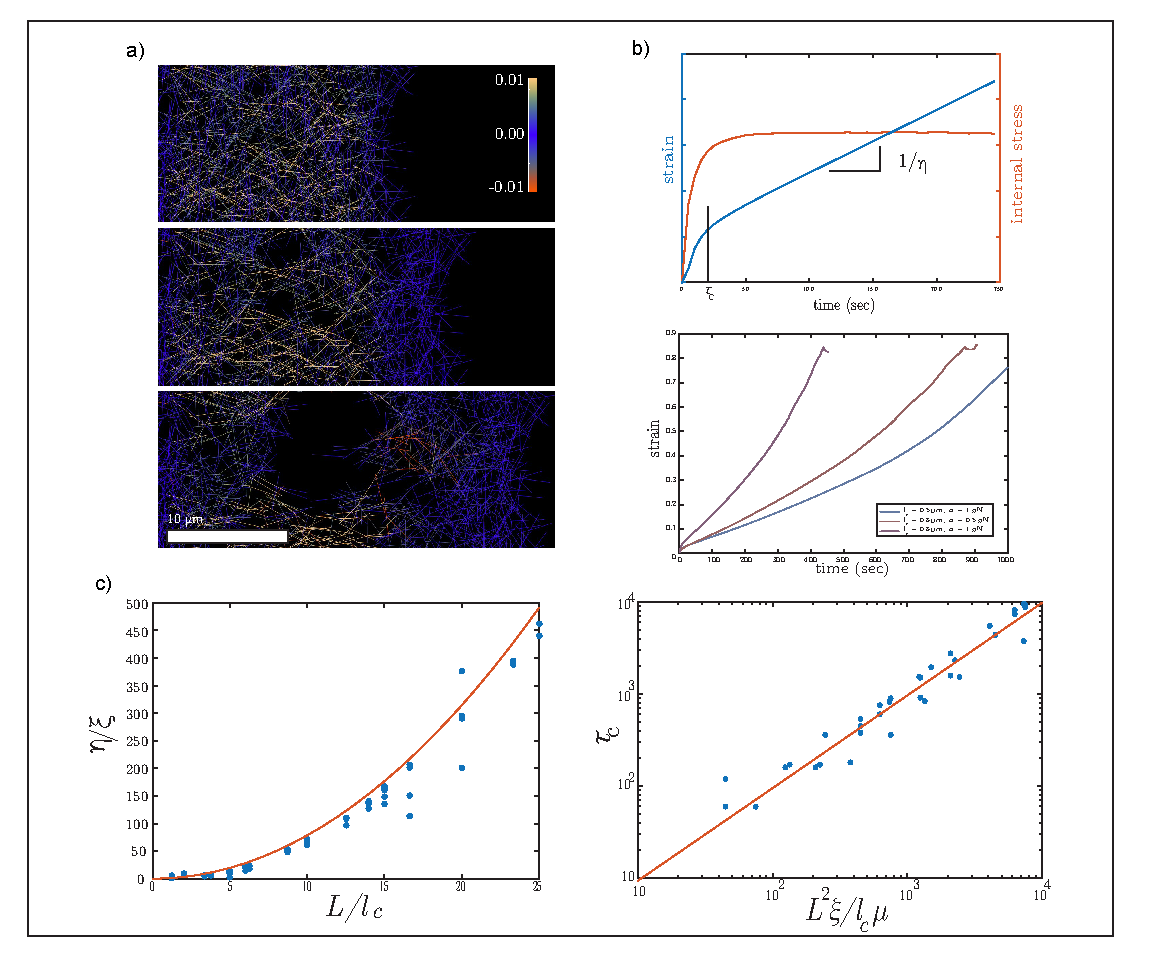
\includegraphics[width=\hsize]{figures/fig3/fig3}
\caption{\label{fig:passive} Filament recycling prevents cortical tearing and modulates the viscous stress relaxation of filament networks under external stress \textbf{a)} Network extension in the presence of cross-link slip alone. i. Example simulations of a network under and external applied extensional stress. ii. Example trace of the stress and strain buildup in an extending network.  The network begins to behave purely viscously at $\tau_c$, and the network deforms like a material with effective viscosity $\eta_c$. iii. The effective viscosity depends on the cross-link drag coefficient and the density of the network. iv. The timescale of the transition to viscous behavior has a characteristic dependence. \textbf{b)} Networks thin and tear at high strains. i. Example simulations of networks under extension at higher strains. ii. Example traces of networks in i.  iii.  Effective viscosity drops as networks are strained. \textbf{c)} Filament recycling rescues network tearing and modulates effective viscosity. i. Examples of same network under extension with and without recycling. ii.  Illustration of the difference in strain for identical network setups in the presence of different filament recycling rates. iii. Master curve for the dependence of filament strain rate on the timescale of filament recycling relative to timescale of cross link slip. }
\end{figure}



\subsection*{Filament recycling allows persistent stress buildup in active networks}

Next we tackled the case of a network with spatially isotropic motor activity.  We found that our simulation axioms were able to produce transient contraction of a patch of free-floating network.  As shown in Figure \ref{fig:active} a, the contraction extent was strongly dependent on the magnitudes of both the filament asymmetry and the motor activity scale.  Additionally, contraction would only occur when there was fractional motor activity, $\phi<1$, (see supplement).  The contraction was able to take place over a time scale, $\tau_c$, but on time scales much longer the contraction would stall and polarity sorting would begin to dominate.

Due to the long term polarity sorting and the fact that filament recycling would be difficult to incorporate into a moving material, we additionally analyzed the stress buildup in a patch that was constrained to maintain its original area.  As shown in Figure \ref{fig:active} b, the results showed a period of net stress due to an imbalance between larger stresses from extended filaments and smaller stresses from compressed filaments.  After a characteristic timescale $\tau_a$, the extensional stress peaks and begins to decrease while the compressive stresses continue to build up resulting in the extensional and compressive stresses beginning to cancel each other.  After another time period, $\tau_{eq}$, the internal stresses become balanced and the net stress drops to approximately 0. The timescale and magnitude of the peak stresses agree with a qualitative expectation discussed later.

Upon the addition of filament recycling, we were able to find that the network maintained a nonzero net stress for times much longer than $\tau_eq$.  We refer to this as the steady state stress because based on our simulations it doesn't appear that this stress ever subsides, and duh.  For similar network parameters as illustrated in Figure \ref{fig:active} c iii, we found that the steady state stress was well predicted by the comparison between the timescale of recycling, $\tau_r$ and that of peak activity, $\tau_a$. 


\begin{figure}[h!]
\centering
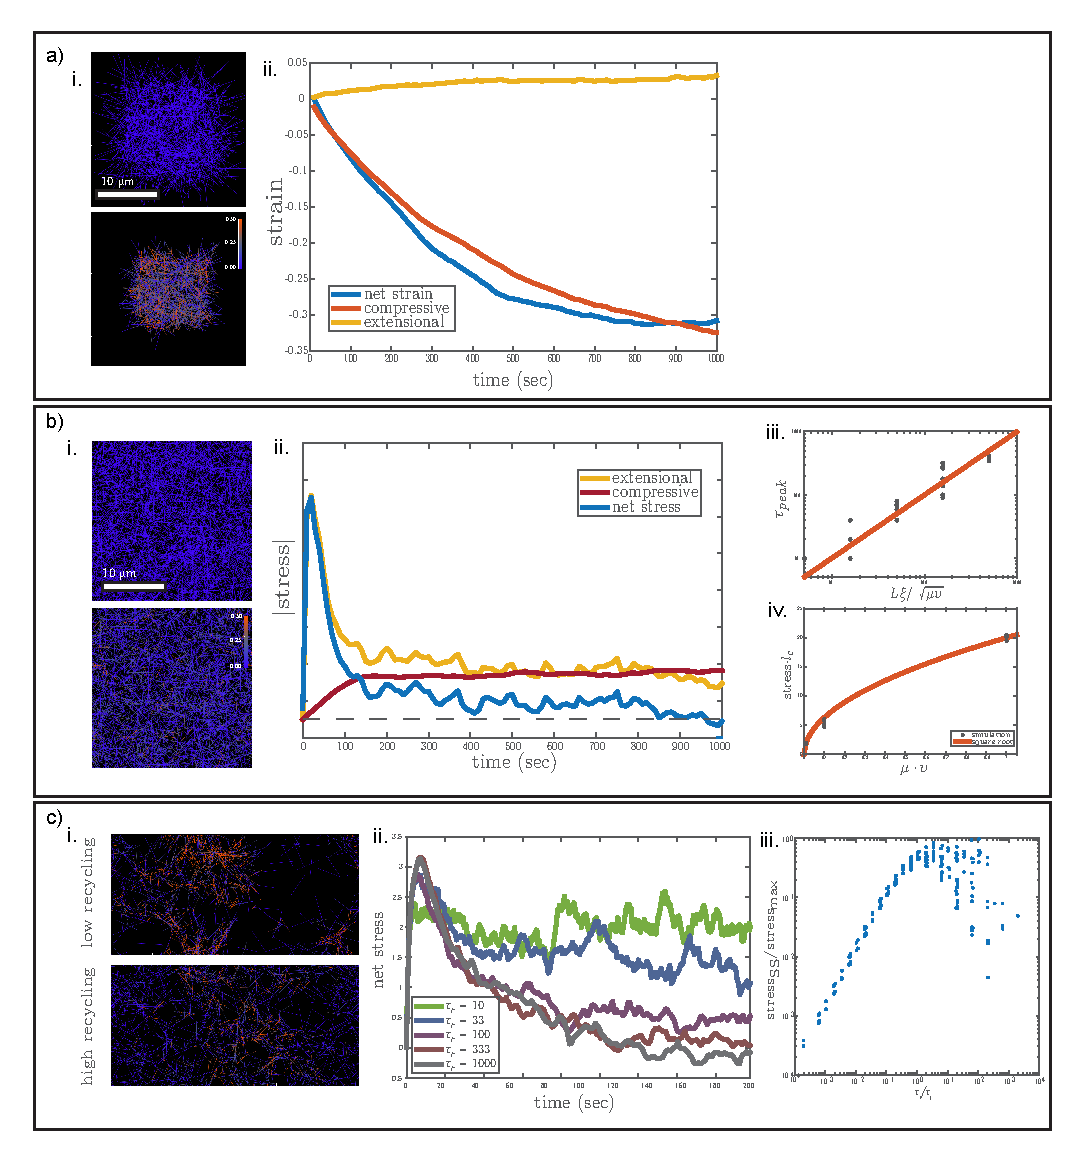
\includegraphics[width=\hsize]{figures/fig4/fig4}
\caption{\label{fig:active} Filament recycling allows persistent active stress buildup in active networks.  \textbf{a)} Network contraction. i. Example of an active network contracting. ii. Traces of total network strain and internal strain of filaments. \textbf{b)} Internal stress buildup is only transient. i. Example simulation of an active network building up internal stress while maintaining a constant area. ii. Traces of stress buildup. iii. Timescale of stress buildup. iv. Peak stress depends on myosin activity and filament stiffness. \textbf{c)} Filament recycling allows for steady state stress buildup. i. Example simulations of networks with fast and slow rates of recycling. ii. Traces of net stress for with different recycling timescales; faster recycling prevents the dress from relaxing entirely.  iii. Steady state stress depends on the recycling time relative to the crossly relaxation time. }
\end{figure}

\subsection*{Filament recycling modulates the balance between active stress buildup and viscous stress relaxation to set the flow rate in polarized networks}











\section*{Supporting Information}

% Include only the SI item label in the subsection heading. Use the \nameref{label} command to cite SI items in the text.

\section*{Acknowledgments}
We would like to thank Shiladitya Banerjee and Patrick McCall for stimulating discussions.

\nolinenumbers

%\section*{References}
% Either type in your references using
% \begin{thebibliography}{}
% \bibitem{}
% Text
% \end{thebibliography}
%
% OR
%
% Compile your BiBTeX database using our plos2015.bst
% style file and paste the contents of your .bbl file
% here.
% 
\bibliographystyle{plos2015}
\bibliography{slippage,active}

\begin{comment}
\begin{thebibliography}{10}
\bibitem{bib1}
Devaraju P, Gulati R, Antony PT, Mithun CB, Negi VS. Susceptibility to SLE in South Indian Tamils may be influenced by genetic selection pressure on TLR2 and TLR9 genes. Mol Immunol. 2014 Nov 22. pii: S0161-5890(14)00313-7. doi: 10.1016/j.molimm.2014.11.005

\bibitem{bib2}
Huynen MMTE, Martens P, Hilderlink HBM. The health impacts of globalisation: a conceptual framework. Global Health. 2005;1: 14. Available: http://www.globalizationandhealth.com/content/1/1/14.

\end{thebibliography}
\end{comment}


\end{document}

